\documentclass{article}

\usepackage[utf8]{inputenc}
\usepackage{enumitem}
\usepackage{amsmath}
\usepackage{amsthm}
\usepackage{amssymb}
\usepackage{graphicx}
\usepackage{tikz}
\usepackage[normalem]{ulem}

\usetikzlibrary{arrows.meta,calc,decorations.pathreplacing,shapes.geometric}
\tikzset{
    >=Stealth,
    er/.style={
        attr/.append style={align=center,draw,thick,ellipse,text width=2cm,text height=1.5ex,text depth=.25ex,font=\strut},
        entity/.append style={align=center,draw,thick,rectangle,text width=2cm,text height=2ex,text depth=.25ex,minimum height=1cm,font=\strut},
        rel/.append style={align=center,draw,thick,diamond,text width=2cm,text height=1.5ex,text depth=.25ex,font=\strut,fill=black!10,scale=0.65},
        isa/.append style={regular polygon, regular polygon sides=3,draw,thick,scale=0.65,font={ISA}},
        total/.append style={ultra thick},
        weak/.append style={ultra thick},
        once/.append style={->},
        strict/.append style={-Arc Barb[]},
        every edge/.append style={draw,thick}
    }
}

\newcommand{\key}[1]{\underline{\smash{#1}}}
\newcommand{\pkey}[1]{\dashuline{\smash{#1}}}
\newcommand{\mname}[1]{\mbox{\sf #1}}
\newcommand{\pnote}[1]{{\langle \text{#1} \rangle}}

\title{Assignment 1}
\author{Hien Tu - tun1}
\date{\today}

\begin{document}

\maketitle

The diagram is given in the ``Assignment 1.png'' file. \\

\textbf{Analysis} \\

The first paragraph of the description is ignored when creating the ER diagram
since it is just an introduction.

The sentence ``First, the system will store information about several cinemas''
indicates that there is an entity Cinema for the diagram. ``Each cinema has a
unique name and an address'' shows that the entity Cinema has attributes name
and address. Although each cinema has a unique name, cinema names have changed
in the past. Thus, we cannot let the attribute name be the primary key. We cannot
let the attribute address be the primary key either since the location of a
cinema may change (e.g., moving the cinema to another place or expanding the
cinema). Thus, I believe it is better to add another attribute called \key{cinema\_id},
stands for cinema id, and let this attribute be the primary key. Therefore, the
Cinema entity has three attributes \key{cinema\_id}, name and address where
\key{cinema\_id} is the primary key.

``Per cinema, the system will also maintain information per room'' illustrates
that the entity Room is owned by the entity Cinema. In other words, Room is a
weak entity of Cinema since a room can only be uniquely defined when there is a
cinema corresponding with it. Since each room has a different room number, the
attribute \pkey{room\_num} is added to be the partial key for the entity Room.
So, the primary key for the entity Room is the pair (\key{cinema\_id}, \pkey{room\_num}).
Based on the  description, the entity also has attributes screen\_type, screen\_size,
projector\_type, sound\_system and accessibility. The examples of screen type,
projector type, sound system are ignored since we focus on the attributes rather
than the examples of each attribute when creating the diagram.

``This information is not only available for cinema visitors, but will also be
communicated to private parties that are looking to hire a room (e.g., for a
corporate event)'' is ignored since the visibility is not restricted to anyone
and also, the database is more for storing data and displaying data should be the
job of another application. ``Finally, per room the system also needs to know the
exact seat arrangement, as the online system will allow customers to order tickets
for specific seats'' indicates that the entity Seat is a weak entity of the entity
Room since seat is a part of the room. The sentence also shows that there is an
entity Ticket that has a relationship with Seat, this will be explain in details
later. The next two sentences of the description show that the entity Seat should
have attributes \pkey{row}, \pkey{seat\_num} and reserved (which means reserved
for disabled people). The reason why we need both \pkey{row} and \pkey{seat\_num}
to be the partial keys is because only the row or only the seat number cannot
uniquely define a seat as one row can have multiple seats and each seat number
will appear in every row, so, we need both to define/locate a seat. Thus, the
primary key for the entity Seat is the 4-tuple (\key{cinema\_id}, \pkey{room\_num},
\pkey{row}, \pkey{seat\_num}).

``Each screening is assigned a single room'' depicts that there is a one-to-many
relationship from an entity Screening to the entity Room. The relationship name
is Room\_Assign and the
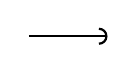
\begin{tikzpicture}[er]
    \path (0,0) edge[strict] (1,0); 
\end{tikzpicture}
arrow from the entity Screening to the relationship Room\_Assign shows that each
screening is associated with exactly one room while the
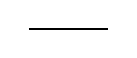
\begin{tikzpicture}[er]
    \path (0,1) edge (1,1);
\end{tikzpicture}
arrow from the entity Room to the relationship Room\_Assign shows that a room
can have multiple screenings. This is the case because each screening only happens
once in exactly one room while one room can have multiple screening (at different
timeslots). The Screening entity has attributes timeslot and screening\_type.
Since timeslot and screening\_type can be the same for different screenings (at
different rooms, for example), we need to have a different, unique attribute for
each screening. We name that atttribute \key{screening\_id}. The explanation of
three types of screening is ignored since it only gives examples for attribute
screening\_type. The explanation on how each screening type affects the ticket
price shows that there should be a relationship between the entities Ticket and
Screening, which will be explained more later. ``For each public screening, the
system keeps track which films are shown. This film information is provided by
the film distributors in a standard format: for now, the system represents this
external information via an entity Film with an attribute fid'' depicts that there
is a relationship between the entity Screening and Film, the relationship is named
Show in the diagram. There is also the entity Film with the primary key attribute
\pkey{fid}, as stated in the description. The relationship between Screening and
Film is many to many since a screening can show multiple films and a film can be
shown in many screenings. ``If a screening will show multiple films (as part of
special screening), then each of these films will be shown in the same room'' is
ingnored because this can be inferred as many films are shown in a screening and
a screening is associated with exactly one room. ``\dots and the
ticket of the customer assign the same seat during each film'' shows that there
is a one to many relationship between an entity Ticket and the entity Seat since
one ticket is only assigned with exactly one seat while one seat can have many
tickets being assigned to (for example, different tickets for different screenings
at the same seat).

``Via an (online) sale, customers can buy one or more tickets for a specific
screening and that are assigned a seat on sale'' first, shows that there is an
entity Ticket (as mentioned before) and an entity Customer. The sentence also
shows that there is a one to many relationship between two entities Ticket and
Screening, namely, Screening\_Assign. Thus, the
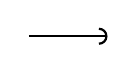
\begin{tikzpicture}[er]
    \path (0,0) edge[strict] (1,0); 
\end{tikzpicture}
arrow is used from Ticket to Screening\_Assign and the
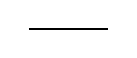
\begin{tikzpicture}[er]
    \path (0,1) edge (1,1);
\end{tikzpicture}
arrow is used from Screening\_Assign to Screening since one ticket can only have
exactly one screening associated with it while one screening can have multiple
tickets associated with it (different people can buy tickets to the same screening).
``Customers that do not feel comfortable with paying online can reserve their
seats online and buy a ticket for these reservations at the counter'' shows that
there should be an attribute reservation to keep track if the ticket is already
paid online or it is a reservation for a seat. The information ``(these reservations
will be cancelled 45 minutes before the start of the film)'' is ignored since
they are to inform when to update the attribute reservation. The next sentence
shows that there should be an attribute mode\_of\_purchase for entity Ticket to
keep track of how they are made. ``whether the sale was related to a reservation''
reassures that there should be an  attribute reservation for the entity Ticket.
Lastly, the attribute price is added to keep track of the paid price. However,
these attributes are not unique, so, we need to define a unique attribute for the
entity Ticket. We name this attribute \key{ticket\_id}.

Furthermore, the sentence ``Via an (online) sale, customers can buy one or more
tickets\dots'' shows that there is an entity Customer and there should be a one
to many relationship, namely, Buy, between Ticket and Customer. Therefore, the
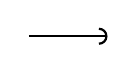
\begin{tikzpicture}[er]
    \path (0,0) edge[strict] (1,0); 
\end{tikzpicture}
arrow points from the entity Ticket to the relationship Buy and the
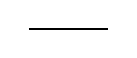
\begin{tikzpicture}[er]
    \path (0,0) edge (1,0); 
\end{tikzpicture}
arrow points from the relationship Buy and the entity Customer since each ticket
can only be bought by one customer but a customer can buy multiple tickets. Since
the description does not mention about the information of the entity Customer,
only a primary key named \key{customer\_id} is added to the entity Customer to
ensure each entity has a primary key.

\end{document}